\chapter{Systemarkitektur}\label{kapitel_Systemark}

\begin{longtabu} to \linewidth{@{}l l l X[j]@{}}
    Version &    Dato &    Ansvarlig &    Beskrivelse\\[-1ex]
    \midrule
    0.1 &    4/11-15 &    Alle &    Tilføjelse af arkitektur\\
    Tekst &    Tekst &    Tekst &    Tekst.\\
    Tekst &    Tekst &    Tekst &    Tekst.\\
    Tekst &    Tekst &    Tekst &    Tekst.\\
\label{version_Systemark}
\end{longtabu}

\textbf{Formål}\\
Til beskrivelse af systemarkitekturen og det detaljerede design for produktet, er der benyttet SysML.
SysML anvendes her, da blodtryksmålesystemet både indeholder software og hardware. Et af de  
vigtigste argumenter for brug af SysML er, at de fastlagte standarder i sproget medfører en bedre 
formidling af systemet, hvilket giver et større overblik.


\section{Hardware}
Hardware-delen består af et elektronisk kredsløb, som forstærker signalet fra tryktransduceren og filtrerer det med et indbygget analogt filter.\\
\newline
Til at skabe overblik over blodtryksmålesystemets hardware er der uarbejdet en figur, der viser hele det overordnet system.

\begin{figure}[H]
\centering
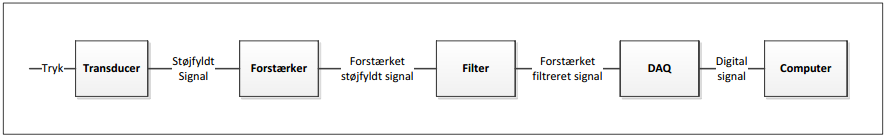
\includegraphics[scale=0.65]{so.PNG}
\caption{Blodtryksmålersystemet}
\end{figure}

Denne illustrerer, at der ind i transduceren kommer tryk og ud kommer et støjfyldt signal. Dette signal bliver ved forstærkeren forstærket og heraf et forstærket støjfyldt signal. Igennem filtret bliver støjen filtreret fra. Det filtrerede signal føres igennem DAQ’en, som omdanner det til et digitalt signal, som anvendes i computerens softwareprogram.\\
\newline
Til at præcisere komponenterne i blodtryksmålesystemets hardware, er der valgt at lave strukturdiagrammer. Her er der anvendt blokdefinitionsdiagram (BDD) og et internt blokdiagram (IBD).

\subsection{BDD}
BDD'et er anvendt til, at dokumentere nedbrydningen af systemet og forholdene mellem blokkene.  

\begin{figure}[H]
\centering
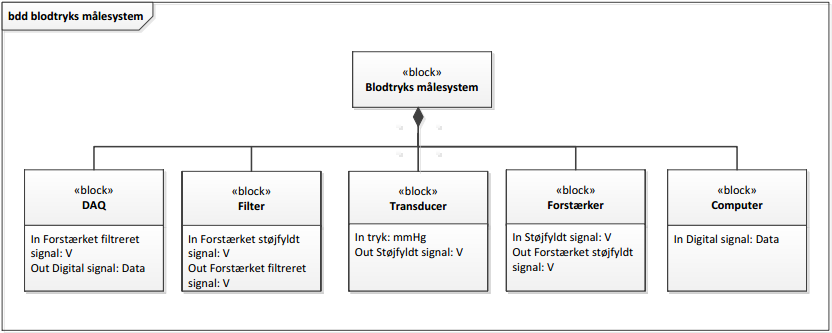
\includegraphics[scale=0.80]{bdd.PNG}
\caption{BDD}
\end{figure}

\textbf{Blokbeskrivelser:}
\begin{itemize}
\item Transducer: En tryktransducer, som konverterer et tryk til et analogt elektrisk signal
\item Forstærker: Signalet forstærkes således at hele forsyningsspændingen udnyttes
\item Filter: Et 2. ordens lavpasfilter fjerner højfrekvent støj
\item DAQ: A/D konverter omsætter den analoge indgangsspænding til et digitalt signal
\item Computer: Enheden som indeholder softwareprogrammet til visning af blodtryk
\end{itemize}
\subsection{IBD}
IBD'et er anvendt til, at dokumentere den interne struktur i blokkene.
\begin{figure}[H]
\centering
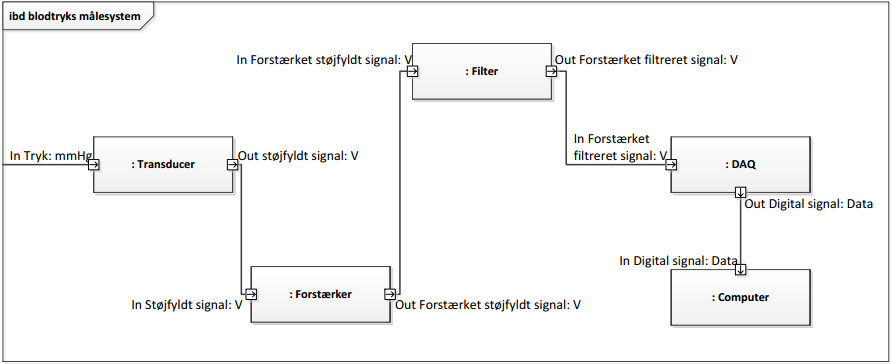
\includegraphics[scale=0.65]{ibd.PNG}
\caption{IBD}
\end{figure}




\subsubsection{Signalbeskrivelse}

\section{Software}
Brugergrænsefladen i software-delen består af to forskellige GUI'er, en til at logge ind og en til diagnostik. Programmet indeholder en række klasser indeholdende funktionaliteten beskrevet i UC's samt databaser til opbevaring af data. Softwaren er opbygget af trelagsmodellen. \\
\newline
For at skabe et overblik over sammenhængen mellem UC's og softwaren i systemet, er der udviklet en applikationsmodel. Applikationsmodellen indeholder en domænemodel over hele systemet, et klassediagram for hver enkelt UC, et sekvensdiagram over hele systemet og et opdateret klassediagram med metoder. Ved at opdele de forskellige dele i software samt at oprette klasser efter den ønskede funktionalitet i UC's, opnås en sammenhænge og overskuelighed over systemet som helhed.
\subsection{Domænemodel}
Domænemodellen er udviklet vha. navneordsanalyse i de fem UC's. Domænemodellen giver et overblik over hvilken funktionalitet der - ud fra UC's - er relevant. Funktionaliteterne er opdelt i kasser, der senere bliver til klasser i softwaren. 

\begin{figure}[H]
\centering
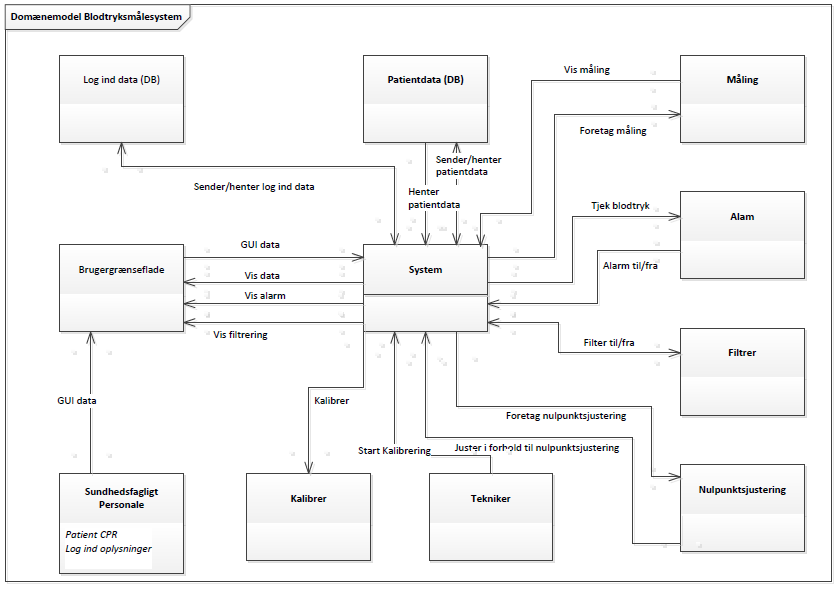
\includegraphics[scale=0.70]{dom.PNG}
\caption{Domænemodel blodtryksmålersystem}
\end{figure}

\subsection{Klassediagram}
%------------UC1----------------------------
\subsubsection{Applikationsmodel UC1}
Klassediagrammet for UC1 
\begin{figure}[H]
\centering
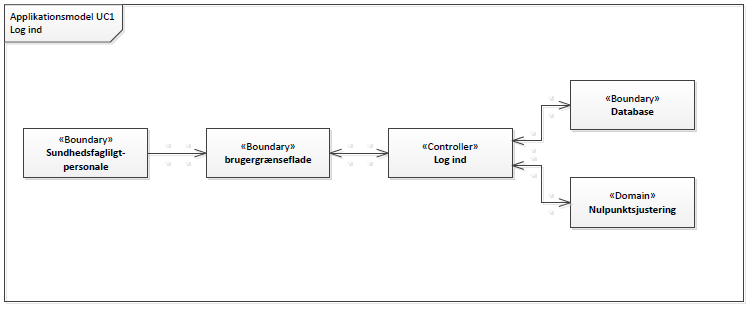
\includegraphics[scale=0.70]{app1.PNG}
\caption{Applikationsmodel UC1}
\end{figure}

%------------------UC2------------------------
\subsubsection{Applikationsmodel UC2}
\begin{figure}[H]
\centering
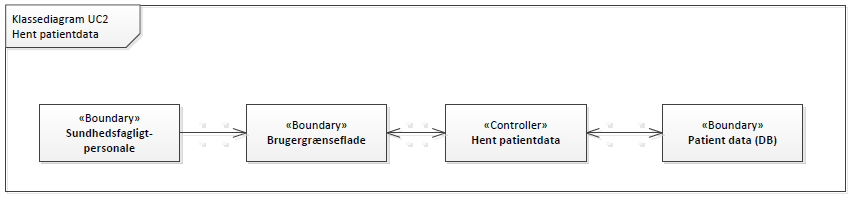
\includegraphics[scale=0.70]{app2.PNG}
\caption{Applikationsmodel UC2}
\end{figure}

%------------------UC3------------------------
\subsubsection{Applikationsmodel UC3}
\begin{figure}[H]
\centering
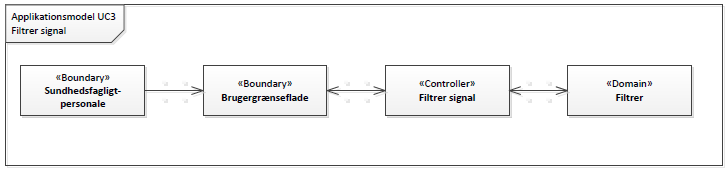
\includegraphics[scale=0.70]{app3.PNG}
\caption{Applikationsmodel UC3}
\end{figure}

%------------------UC4------------------------
\subsubsection{Applikationsmodel UC4}
\begin{figure}[H]
\centering
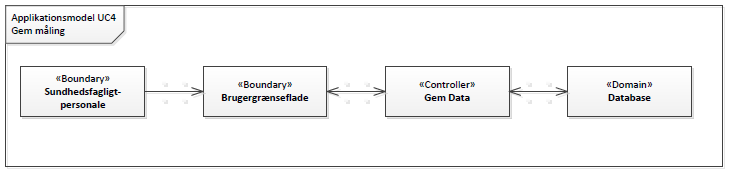
\includegraphics[scale=0.70]{app4.PNG}
\caption{Applikationsmodel UC4}
\end{figure}

%------------------UC5------------------------
\subsubsection{Applikationsmodel UC5}
\begin{figure}[H]
\centering
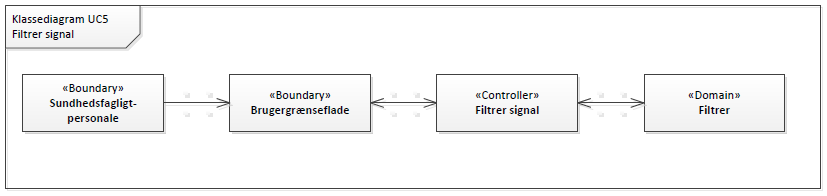
\includegraphics[scale=0.70]{app5.PNG}
\caption{Applikationsmodel UC5}
\end{figure}

